
% -----------------------------------------------------------------------------
% Auteurs : Romain de Wolff, Bruno da Silva, Gilles Meier
% -----------------------------------------------------------------------------
\documentclass[10pt,a4paper,titlepage]{article}
\usepackage[utf8]{inputenc}     % encodage des characteres en utf8
\usepackage[francais]{babel} % pour la table des matières en français 

\usepackage{url} % pour les liens internet
\usepackage[colorlinks=true,linkcolor=black,bookmarks=true,bookmarksopen=true]{hyperref} % rendre les liens clickable
\usepackage{fancyhdr}	 
\usepackage{listings} 
\lstset{language=Java, breaklines, fontadjust, inputencoding=utf8, basicstyle=\small, numbers=left, numberstyle=\tiny, tabsize=2}

\usepackage[dvips]{graphicx}
\usepackage{epstopdf}
\usepackage[parfill]{parskip}             % Activate to begin paragraphs with an empty line rather than an indent
\usepackage{pdfpages} % pour inclure des fichiers PDF : commande \includepdf[pages=-]{votre_fichier} 


% -----------------------------------------------------------------------------
%   Info sur le labo
% -----------------------------------------------------------------------------
\newcommand{\branchetag}{ASI}
\newcommand{\branche}{Applications et Services Internet}
% \newcommand{\labonummer}{}
\newcommand{\laboname}{Laboratoire SSL avec JSSE}
\newcommand{\auteurOne}{Romain de Wolff \\ Simon Hintermann}
% \newcommand{\auteurTwo}{Bruno da Silva}
\newcommand{\promo}{IL2008}
\newcommand{\titreDocument}{Rapport de laboratoire}
% -----------------------------------------------------------------------------


% -----------------------------------------------------------------------------
% Pour l'utilisation de code
% -----------------------------------------------------------------------------
\usepackage{listings} 
%\lstset{language=Java, breaklines, fontadjust, inputencoding=utf8, basicstyle=\small, numbers=left, numberstyle=\tiny, tabsize=2}

\usepackage{courier}
\usepackage{color}

% color definitions
\definecolor{dkgreen}{rgb}{0,0.6,0}
\definecolor{gray}{rgb}{0.5,0.5,0.5}
\definecolor{lightblue}{rgb}{0.92,0.92,1}

\lstset{language=Html,
  %keywords={break,case,catch,continue,else,elseif,end,for,function,
  %   global,if,otherwise,persistent,return,switch,try,while},
  keywords={script, document, function},
  %basicstyle=\ttfamily\small,
  basicstyle=\scriptsize,
  keywordstyle=\color{blue},
  commentstyle=\color{dkgreen},
  stringstyle=\color{red},
  numbers=none,
  numberstyle=\tiny\color{gray},
  stepnumber=1,
  numbersep=10pt,
  backgroundcolor=\color{lightblue},
  tabsize=2,
  linewidth=0pt,
  showspaces=false,
  showstringspaces=false,
  frame=single,
  framexleftmargin=10pt,
  framexrightmargin=10pt,
  framexbottommargin=7pt,
  framextopmargin=7pt,
  linewidth=335pt, % largeur de la ligne de code affichée
  xleftmargin=10pt, % espace avant le debut du cadre
  aboveskip=20pt
}
% -----------------------------------------------------------------------------
% En tete et pied de page

\pagestyle{fancy} % defini nos propre header & footer
\fancyhf{} % delete current header and footer 
\fancyhead[L]{\branchetag}
\fancyhead[C]{\laboname}
\fancyhead[R]{\auteurOne} 
\fancyfoot[L]{
\includegraphics[width=3cm]{img/HEIG-VD.jpg}}
\fancyfoot[R]{\bfseries\thepage}

\renewcommand{\headrulewidth}{0.5pt} 
\renewcommand{\footrulewidth}{0.1pt} 
\addtolength{\footskip}{10.0pt} % space for the rule 
\fancypagestyle{plain}{
	\fancyhead{} % get rid of headers on plain pages 
	\fancyfoot{}
	\renewcommand{\headrulewidth}{0pt} % and the line 
	\renewcommand{\footrulewidth}{0pt} % and the line 
}

\author{\auteurOne}
\title{\branchetag : \laboname}
\date{\today}

\begin{document}
% -----------------------------------------------------------------------------
% Page de titre
\pagenumbering{Roman}
\pagestyle{headings}
\begin{titlepage}
	\begin{center}

		
\includegraphics[width=6cm]{img/HEIG-VD.jpg}

		\vspace{3cm}
		\LARGE \branche %Laboratoire No %\labonummer \\
		\vspace{3cm}\\
		\Huge \laboname \\
		\vspace{3cm}

		\Large \textsc{\titreDocument} \\
		\vspace{3cm}

		\large \auteurOne \\
		% \auteurTwo \\ % pour un eventuelle deuxième auteur
		\vspace{10pt}
		\normalsize \textsc{\promo} \\
		\vspace{1cm}
		\today
	\end{center}
\end{titlepage}
% -----------------------------------------------------------------------------

% -----------------------------------------------------------------------------
% Table des matières
\tableofcontents
\newpage
\pagestyle{fancy}
\pagenumbering{arabic}
 
% -----------------------------------------------------------------------------
\section{Introduction}
% -----------------------------------------------------------------------------

Le but de ce laboratoire est de modifier le serveur web créé en Java durant un laboratoire précédant et d'y implémenter le protocole SSL/TLS. Notre serveur web doit se lancer dans deux mode différent: un mode avec authentification du client nécessaire et un autre sans. 

Durant ce laboratoire, nous nous sommes basé sur le serveur web de M. Maulini. 

% -----------------------------------------------------------------------------
\section{Utilisation du serveur web}
% -----------------------------------------------------------------------------

Le lancement du serveur s'effectue à l'aide de la ligne de commande. Pour lancer le serveur avec authentification du client sur le port 443 (port par défaut de SSL) il faut utiliser la commande suivante:

\lstset{frameround=fttt}
\begin{lstlisting}[frame=trBL]
	java WebServer 1 443
\end{lstlisting}

Le “1” permet de dire que l'on active l'authentification du client. Pour le rendre facultatif, on utilisera un “0” à la place, comme le montre la commande suivante:

\begin{lstlisting}[frame=trBL]
	java WebServer 0 443
\end{lstlisting}

Notons que pour lancer le serveur sur le port 443 comme montré ci dessus il faut exécuter la commande en tant qu'administrateur du système. 





% -----------------------------------------------------------------------------
\section{Clé publique générée}
% -----------------------------------------------------------------------------

Voici la clé publique qui nous a été generée par Keytool :

{\scriptsize
\begin{verbatim}
-----BEGIN NEW CERTIFICATE REQUEST-----
MIIBujCCASMCAQAwejELMAkGA1UEBhMCQ0gxCzAJBgNVBAgTAlZEMREwDwYDVQQHEwhMYXVzYW5u
ZTEZMBcGA1UEChMQd3d3LlRBR0FEQVJULmNvbTEcMBoGA1UECxMTUGVyc29uYWwgV2ViIFNlcnZl
cjESMBAGA1UEAxMJMTI3LjAuMC4xMIGfMA0GCSqGSIb3DQEBAQUAA4GNADCBiQKBgQCjcLrCVl/h
50CuSHjNevhTrRS0bCQ1oCN27c3hTLdDbLVjDNqUJqziTXpowFTUXmM/hrbKwVzM5+I4krwx/6dW
oVVhaGywxkQwN4mQ2rgFvkdm8xIpPKfyVMTLYRQLfd89qLYC8C0SUR3MqzuNRpT7lnla1RB9A6Mg
IIx53mf8UQIDAQABoAAwDQYJKoZIhvcNAQEEBQADgYEAAht/hvwHdT1Qb5ZPe6EmBbMJe6VozqQT
yzaA2q6+4Y+FzuQ0PT7oePyg22e6HTiEtxRIhNGiCXVlceeNxKYFBGoBGVSGOHvauWFGRntErntQ
X7vYKW5XCjHfEpsMwKsj42b4zMFn743IT/LmiC/NsghW3q+UD7AUslld4+XaX68=
-----END NEW CERTIFICATE REQUEST-----
\end{verbatim}
}


% -----------------------------------------------------------------------------
\section{Réponses aux questions}
% -----------------------------------------------------------------------------

Lors de la connexion sur notre serveur HTTPS à l'aide du navigateur Firefox, le serveur nous affiche une alerte comme le montre la figure \ref{fig:connex}

\begin{figure}[htbp]
   \begin{center}
      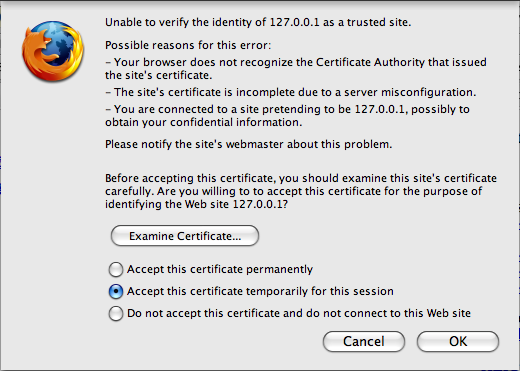
\includegraphics[width=345px]{img/1.png}
   \end{center}
   \caption{Alerte affichée lors de la connexion sur le site sécurisé.}
	\label{fig:connex}
\end{figure}

Nous acceptons ce certificat et nous allons voir le site s'afficher. On remarque que le site est sécurisé grâce à l'icône représentant un cadenas (an bas à droite dans Firefox) que l'on peut voire sur la figure \ref{fig:icone}.

\begin{figure}[htbp]
   \begin{center}
      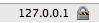
\includegraphics[height=23px]{img/2.png}
   \end{center}
   \caption{Icone dans la barre des tâches du navigateur Firefox.}
	\label{fig:icone}
\end{figure}

En cliquant sur le cadenas on peut afficher les informations relatives à la sécurité et donc du certificat que l'on a accepté. La figure \ref{fig:infosecu} nous montre à quoi ressemble cette fenêtre.

\begin{figure}[htbp]
   \begin{center}
      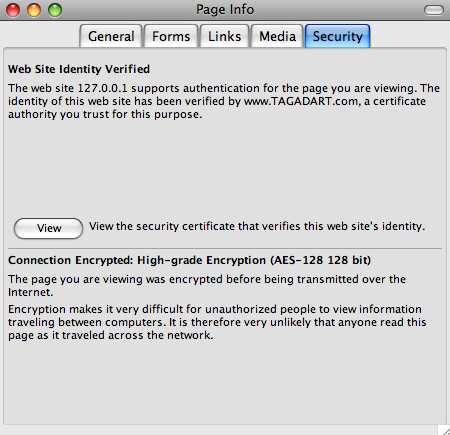
\includegraphics[width=345px]{img/3.png}
   \end{center}
   \caption{Information sur la sécurité du site.}
	\label{fig:infosecu}
\end{figure}

La figure \ref{fig:infosecu} nous montre les informations sur le certificat et nous avertit que nous faisons confiance au CA mentionné. En cliquant sur le bouton “View” on obtient les informations sur le certificat, exactement les informations que nous avons introduites lors de la création à l'aide de \emph{Keytool}. La figure \ref{fig:certif} nous montre cette fenêtre.

\begin{figure}[htbp]
   \begin{center}
      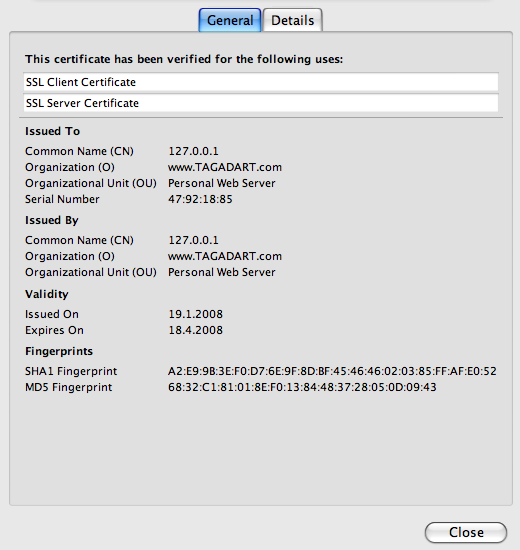
\includegraphics[width=345px]{img/4.png}
   \end{center}
   \caption{Affichage détaillée des informations sur le certificats que nous avons créé.}
	\label{fig:certif}
\end{figure}

\subsection{En examinant le certificat du serveur, comment pouvez-vous en déduire que celui-ci est auto-signé?}

On le voit bien sur la figure \ref{fig:certif}: les champs “Issued To” (distribué à)  et “Issued By” (distribué par) sont identiques. On sait dès lors que le certificat est auto-signé. Certain navigateur affiche même directement l'information “Certificat Auto-Signé”. C'est le cas notamment de Safari sous Mac OS X.

\subsection{Pourquoi serait-il intéressant de faire signer le certificat par une entité comme Verisign?}

Verisign est une autorité de certification (CA): elle émet des certificats qu'elle vends. Ces certificats sont réputés fiable. L'avantage d'avoir un certificat d'un CA reconnue est que les utilisateurs qui se connecte sur le site peuvent, grâce à la renomée de Verisign, savoir que le site a identifié une entité correctement. C'est donc pour des questions de sécurité et de véracité que nous avons avantage à utiliser les services offert par une société comme Verisign.

L'utilisateur sera donc mis en confiance et, surtout, n'aura pas d'avertissement du navigateur comme quoi le certificat est douteux. 

% -----------------------------------------------------------------------------
\section{Observations}
% -----------------------------------------------------------------------------

Nous allons établir deux connexions avec le serveur web et les comparer. La première sans authentification du client et la seconde avec. L'annexe 1, “Communication SSL” illustre, par un diagramme en flèches, les échanges entre le client et le serveur. Des numéros y figurent auxquelles nous ferons référence lors de nos explications.

Nous allons suivre le déroulement partiel des deux type de connexions. Les captures du logiciel Wireshark sont incluses afin de bien voir ce qu'il se passe lors de la connexion. 

Les premiers message échangé (1) font partie du \emph{3 way handshake}. C'est à ce moment que le navigateur web (dans notre exemple Firefox) établit une connexion avec le serveur. Ces messages ne sont pas propres à SSL mais il est intéressant de les mentionner ici.

Le client envoie un message \texttt{Client Hello} (2) qui contient la liste des algorithmes et la dernière version de SSL qu'il supporte.

Le serveur effectue les choix du \emph{cipher} ainsi que la version de SSL, la plus récente possible, qu'ils utiliseront pour communiquer.

Le dernier message identique échangé est \texttt{Certificate} que le serveur envoie au client. Il est optionnel lorsque l'authentification du client n'est pas nécessaire mais indispensable si l'on désire authentifier le client.

La étapes suivantes changent en fonction du système d'authentification choisit.

\subsection{Connexion sans l'authentification client}

\begin{figure}[htbp]
   \begin{center}
      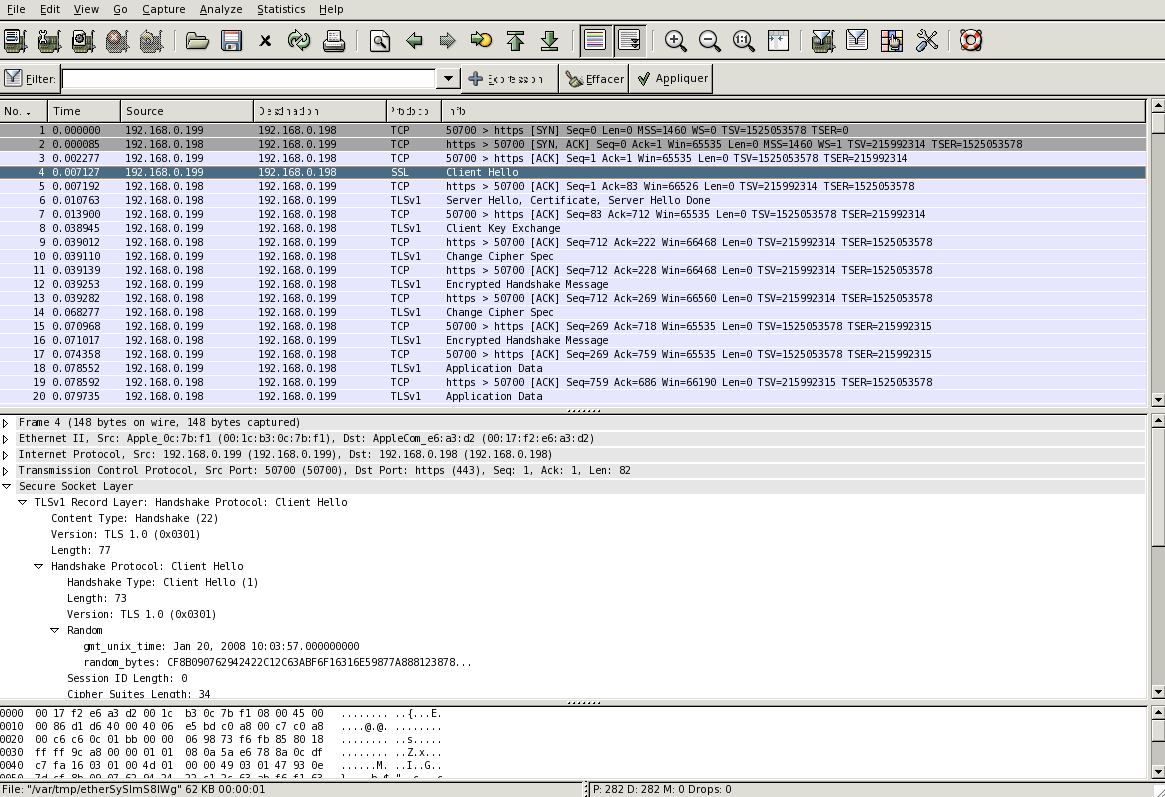
\includegraphics[width=345px]{img/wireshark-nouser-auth.png}
   \end{center}
   \caption{Logiciel de capture de paquet Wireshark, communication client-serveur \underline{sans} authentification du client.}
	\label{fig:wireshark-nouserauth}
\end{figure}

Si l'authentification du client n'est pas nécessaire, le message suivant est \texttt{Server Hello Done} (5), envoyé par le serveur. Il permet d'indiquer au client que les négociations initiales sont terminées de son côté. 

Dans les étapes suivantes, le client va échanger des informations pour permettre de créer les clés symétriques (6, \texttt{Client Key Exchange}). Une fois la clé symétrique partagée, le client demande de passer mode sécurisé (7, \texttt{Change Cipher Spec}). Le serveur envoie aussi (8) un message \texttt{Change Cipher Spec} qui va permettre finalement de communiquer de manière chiffrée. C'est les message de type \texttt{Application Data} qui contiennent les données chiffrées transmises entre le client et le serveur.

\subsection{Connexion avec l'authentification client activée}

Si l'authentification du client est demandée par le serveur, ce dernier va envoyer au client un message \texttt{Certificate Request} (4). Le serveur demande au client de lui envoyer son certificat afin de pouvoir décider si il pourra se connecter ou non.

Le client envoie alors son certificat (9) que le serveur peut vérifier. 

Les autres message échangé sont identiques que la version qui ne demande pas d'authentification à l'utilisateur. La négociation et le changement pour passer en mode chiffré se font de la même manière.

Dans le cas ou la connexion s'établit correctement, les échanges de messages se déroulent comme illustrés sur la figure \ref{fig:wireshark-userauthOk}. Si au contraire, le client est rejeté, la communication sera brutalement interrompue comme illustré sur la figure \ref{fig:wireshark-userauthError}.

\begin{figure}[htbp]
   \begin{center}
      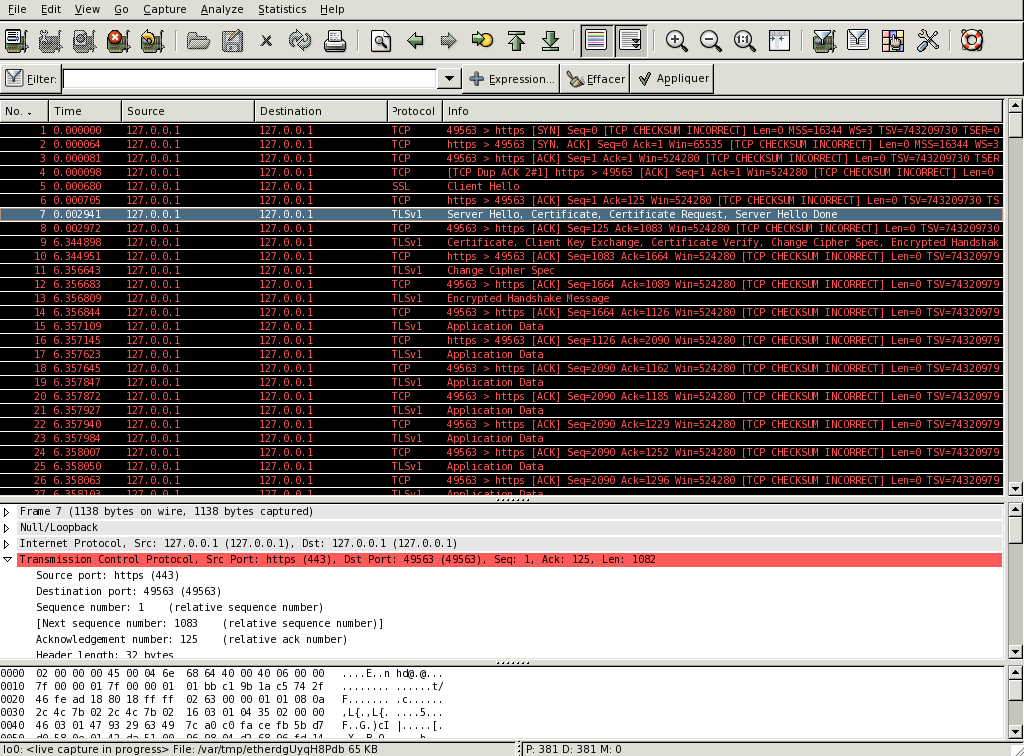
\includegraphics[width=345px]{img/wireshark-with-auth-OK.png}
   \end{center}
   \caption{Logiciel de capture de paquet Wireshark, communication client-serveur \underline{avec} authentification du client (connexion OK).}
	\label{fig:wireshark-userauthOk}
\end{figure}

\begin{figure}[htbp]
   \begin{center}
      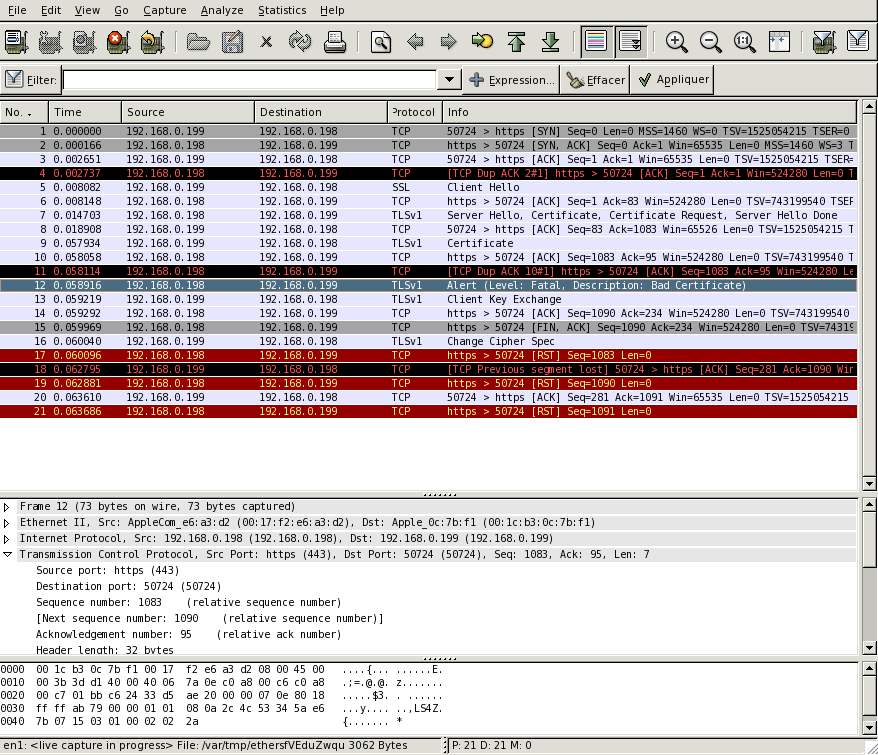
\includegraphics[width=345px]{img/wireshark-with-auth-ERROR.png}
   \end{center}
   \caption{Logiciel de capture de paquet Wireshark, communication client-serveur avec authentification du client et erreur (le client ne possède pas le certificat).}
	\label{fig:wireshark-userauthError}
\end{figure}

\subsection{Cipher utilisé}

La figure \ref{fig:wireshark-cipher} nous montre clairement que le cipher utilisé pour la communication entre le client et le serveur est \texttt{TLS\_RSA\_WITH\_RC4\_128\_MD5}. Le crypthosystème utilisé correspond à celui le plus élevé compatible par le client et le serveur. Le système utilisé variera donc en fonction de ce que supporte le client et le serveur.

\begin{figure}[htbp]
   \begin{center}
      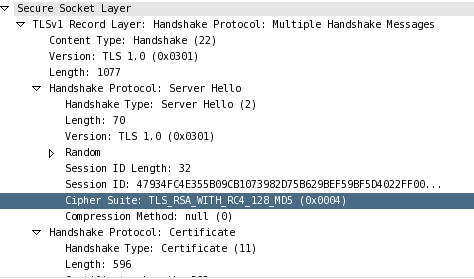
\includegraphics[width=345px]{img/selected-cipher.png}
   \end{center}
   \caption{Selection du cipher utilisé lors de la communication SSL entre le client et le serveur}
	\label{fig:wireshark-cipher}
\end{figure}

Dans la classe \texttt{WebServer.java}, nous pouvons changer la liste des \emph{ciphers} utilisé par notre serveur grâce à la constante \texttt{CIPHERSUITES}.

\begin{lstlisting}[frame=trBL]
	final static String[] CIPHERSUITES = {
		"SSL_RSA_WITH_3DES_EDE_CBC_SHA",  
		"SSL_RSA_WITH_RC4_128_SHA",
		"SSL_RSA_WITH_RC4_128_MD5"
	};
\end{lstlisting}

\subsection{Principales différences entre SSL v3 et TLS v1}

Pour force l'utilisation de l'une ou l'autre des spécifications, on peut modifier l'objet \texttt{SSLContext} comme cela :

\begin{lstlisting}[frame=trBL]
SSLContext sslContext = SSLContext.getInstance("TLS");
\end{lstlisting}

Ici on a choisit \texttt{TLS}, mais on peut aussi choisir \texttt{SSLv3}. On a récupéré ces informations grâce aux méthodes \texttt{getEnabledProtocls()} et \texttt{getEnabledCipherSuites()}. Nous les affichons dans la console dont voici un extrait : 

\begin{verbatim}
	********************************************
	Enabled Session Creation ? false
	Protocols actifs:
	 - SSLv2Hello
	 - SSLv3
	 - TLSv1
	Ciphers actifs:
	 - SSL_RSA_WITH_3DES_EDE_CBC_SHA
	 - SSL_RSA_WITH_RC4_128_SHA
	 - SSL_RSA_WITH_RC4_128_MD5
	********************************************
\end{verbatim}

Selon la documentation que nous avons trouvé sur internet, il semble que les différences entre SSLv3 et TLS sont minimes. On note quand même que ces deux protocole ne sont pas compatibles dans les deux sens, mais que TLS soit compatible avec SSL v3.

\subsection{Le message \emph{Certificate Verifiy}}

Le message \texttt{Certificate Verify} est utile lorsque l'on désire authentifier le client. Pour se faire, le client signe numériquement à l'aide de sa clé privée ceci afin que le serveur puisse vérifier son identité. Le serveur pourra la vérifier en utilisant la clé publique du client.

\subsection{Configuration du serveur web avec système d'authentification mais sans chiffrement de données}

Pour que notre serveur web effectue uniquement de l'authentification, il faut le lancer avec authentification du client et modifier l'objet \texttt{serveur} appartenant à la classe \texttt{SSLServerSocket}. La méthode \texttt{setEnableSessionCreation()} permet d'effectuer cette action.

En effet, si la session n'est pas créée, on aura uniquement l'authentification qui sera effectuée. Le reste des communications ne sera pas chiffrés.

L'autre moyen décrit dans le cours, permet de désactivé le chiffrement des données en changeant le type de cipher utilisé. En effet, la structure des ciphers permet de contrôler le chiffrement utilisé.

Nous pouvons ainsi désactiver le chiffrement de donnée en insérant \texttt{NULL} à la place de l'option de chiffrement de session.

\begin{lstlisting}
SSL_RSA_WITH_3DES_EDE_CBC_SHA
\end{lstlisting}

devient

\begin{lstlisting}
SSL_RSA_WITH_NULL_SHA
\end{lstlisting}

Nous avons donc deux moyens de ne pas chiffrer les données transmises durant la session. 

% -----------------------------------------------------------------------------
\section{Conclusion}
% -----------------------------------------------------------------------------

La découverte et l'implémentation du protocole SSL/TLS est passionnant. Nous n'avions jamais effectué de serveur sécurisé de cette manière. Le langage Java qui met à disposition JSSE nous facilite grandement la vie et rend la création d'un serveur web sécurisé relativement facile. 

Après avoir lus la documentation et fait quelques tests, il nous fallut simplement du temps pour faire tout ce qui est demandé dans ce laboratoire et aucunes difficulté particulière n'est survenue.

% -----------------------------------------------------------------------------
\section{Références}
% -----------------------------------------------------------------------------

{\scriptsize
\begin{description}
	\item[\url{http://www.ietf.org/rfc/rfc2246.txt}] TLS Specifications, IETF
	\item[\url{http://wp.netscape.com/eng/ssl3/draft302.txt}] SSL v3 Specifications, Netscape
	\item[\url{http://java.sun.com/javase/6/docs/technotes/guides/security/jsse/JSSERefGuide.html}]	Java Secure Socket Extension (JSSE) - Reference Guide, Sun.com
	\item[\url{http://java.sun.com/javase/technologies/security/}] Java SE Security, Sun.com
	\item[\url{http://fr.wikipedia.org/wiki/Transport_Layer_Security}] {TLS et SSL, Wikipedia.org}
	\item[\url{http://www.javaworld.com/javatips/jw-javatip115.html}] Secure JavaMail with SSL, JavaWorld.com
	\item[\url{http://publib.boulder.ibm.com/infocenter/tivihelp/v2r1/index.jsp?topic=/com.ibm.itame2.doc_5.1/ss7aumst18.htm}] The SSL Handshake, IBM.com
	\item[\url{http://www.commentcamarche.net/crypto/ssl.php3}] Cryptographie SSL, CommentCaMarche.net
	\item[\url{http://www.computing.net/webdevel/wwwboard/forum/439.html}] SSL vs TLS, Forum Computing.Net
\end{description}
}

% -----------------------------------------------------------------------------
\section{Annexe}
% -----------------------------------------------------------------------------

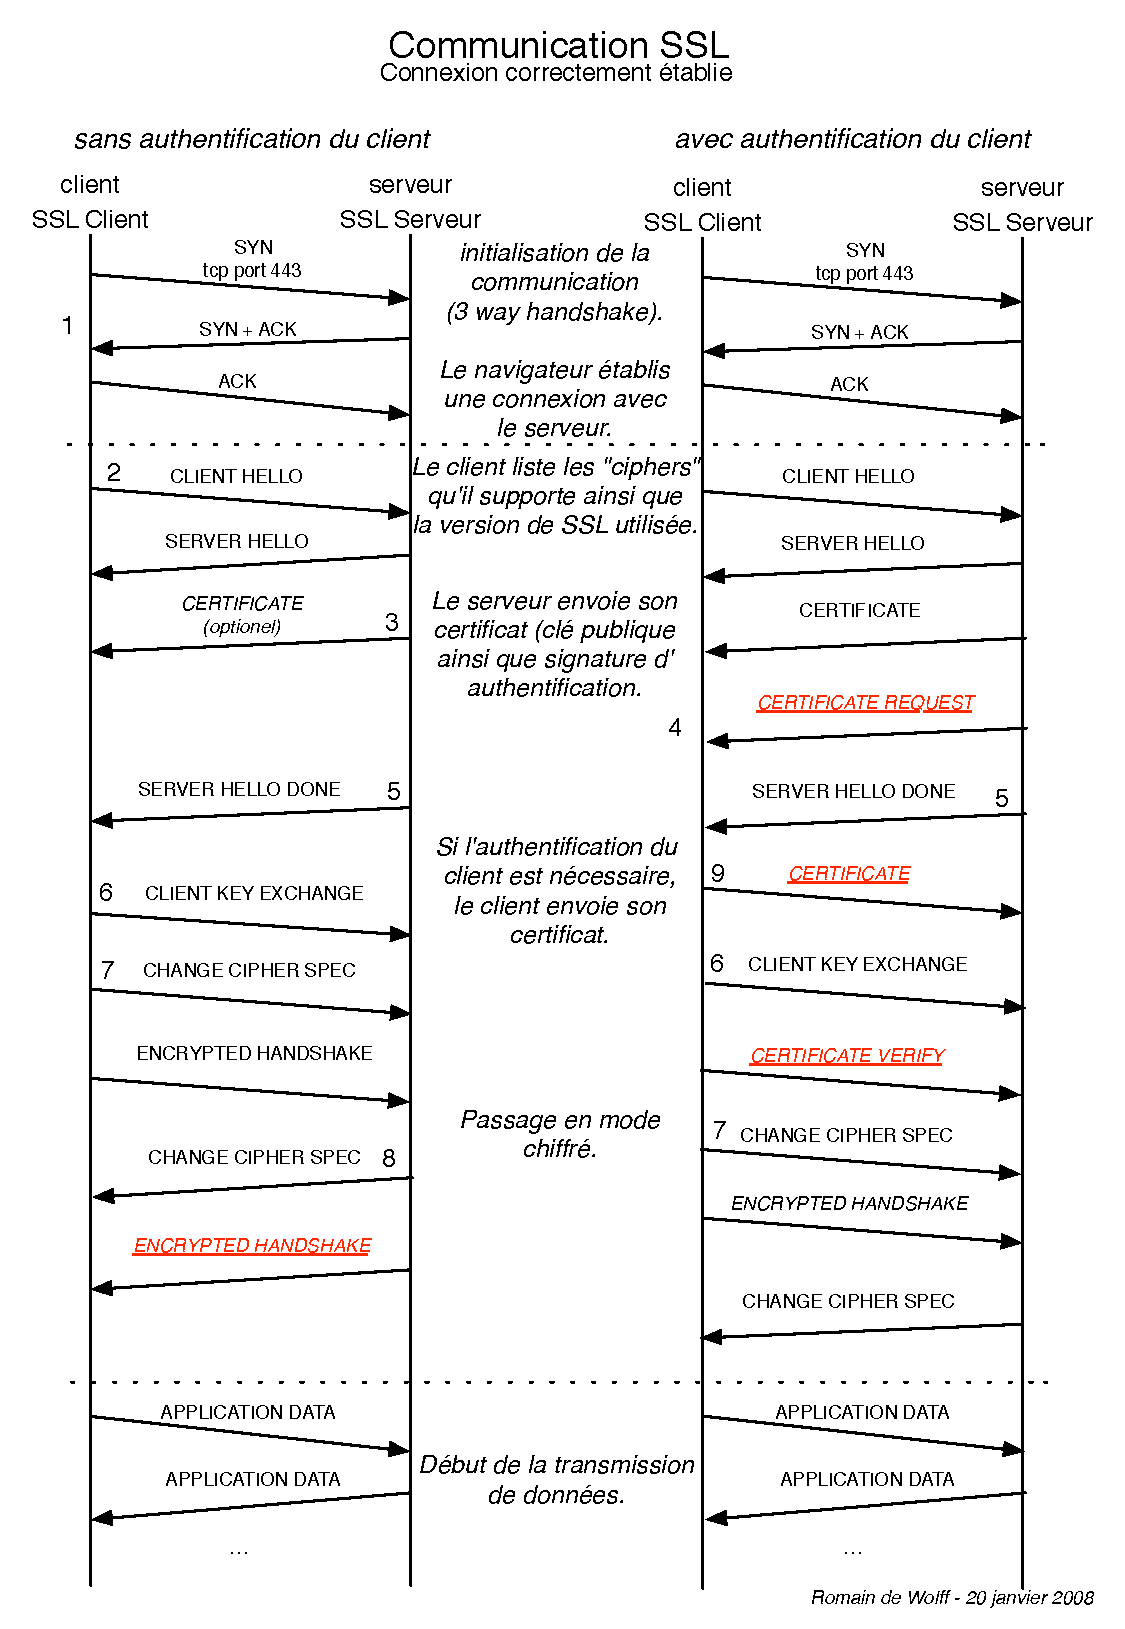
\includegraphics[width=12cm]{CommunicationSSL.pdf} 


\end{document}